\documentclass[english]{article}

%% Packages pull in extra commands:
%% http://en.wikibooks.org/wiki/LaTeX/Packages

\usepackage{hyperref}
\usepackage[letterpaper]{geometry}
\geometry{verbose,tmargin=1in,bmargin=1in,lmargin=1in,rmargin=1in}
\usepackage{amsmath}
\usepackage{amssymb}
\usepackage{graphicx}
\usepackage{float}
\usepackage{array}
\usepackage{tikz}
\usepackage{enumitem}
\usepackage{bbm}
\usepackage{xspace}
\DeclareMathOperator*{\argmax}{argmax}
\usepackage{spverbatim}
\usepackage{hyperref}

% New commands serve as shorthand for frequently used command combinations.
\newcommand{\ind}[1]{\mathbf{1}\left(#1\right)}
\newcommand{\bx}{\mathbf{x}}
\newcommand{\E}{\mathbf{E}}
\newcommand{\MATLAB}{\textsc{Matlab}\xspace}
\newcommand\scalemath[2]{\scalebox{#1}{\mbox{\ensuremath{\displaystyle #2}}}}

\title{CIS581: Project 3\\Part A: Image Stitching\\Due: Nov. 1, 2018 at 11:59 pm}
\author{Wentao He}

\begin{document}
\maketitle
\section{Input Images}
In this project, I used in total of three images for mosaicing: \texttt{boat1.jpg}, \texttt{boat2.jpg} and \texttt{boat3.jpg}, which are shown in Figure \ref{fig:boat1}, Figure \ref{fig:boat2}, and Figure \ref{fig:boat3}.
        \begin{figure}[H]
          \centering
          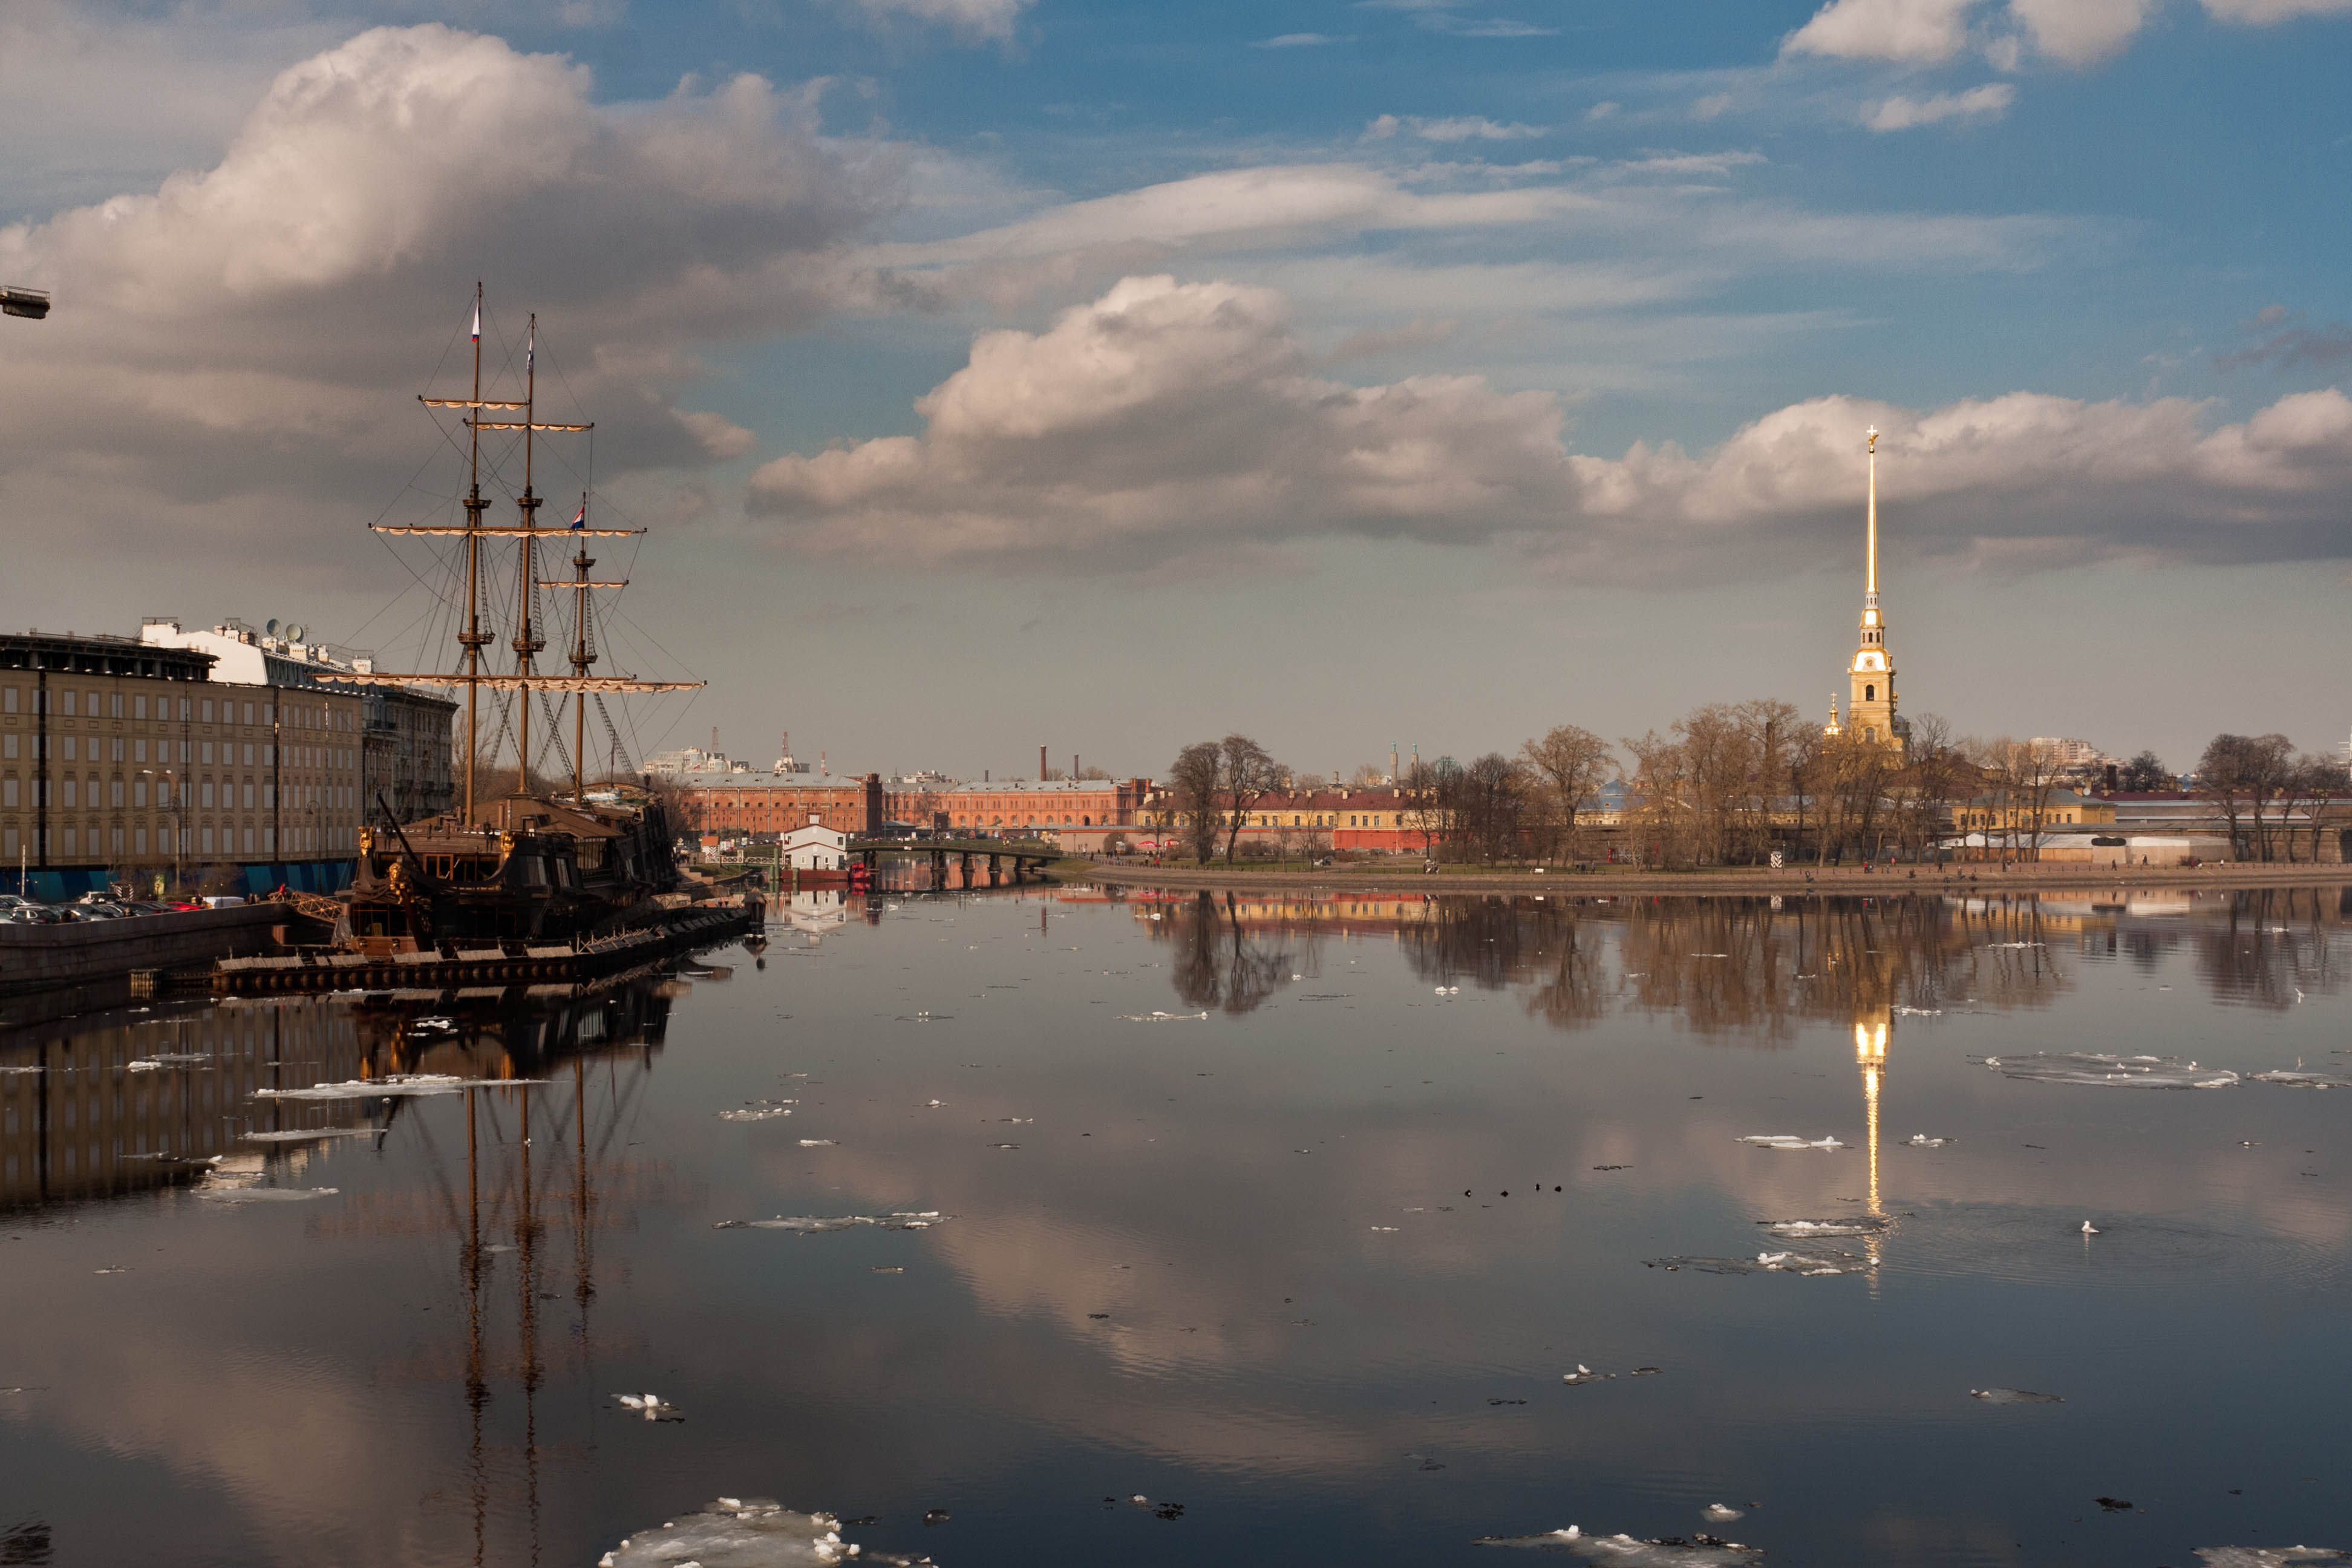
\includegraphics[width=1\textwidth]{boat1.jpg}
          \caption{boat1.jpg}
          \label{fig:boat1}
        \end{figure}
        \begin{figure}[H]
          \centering
          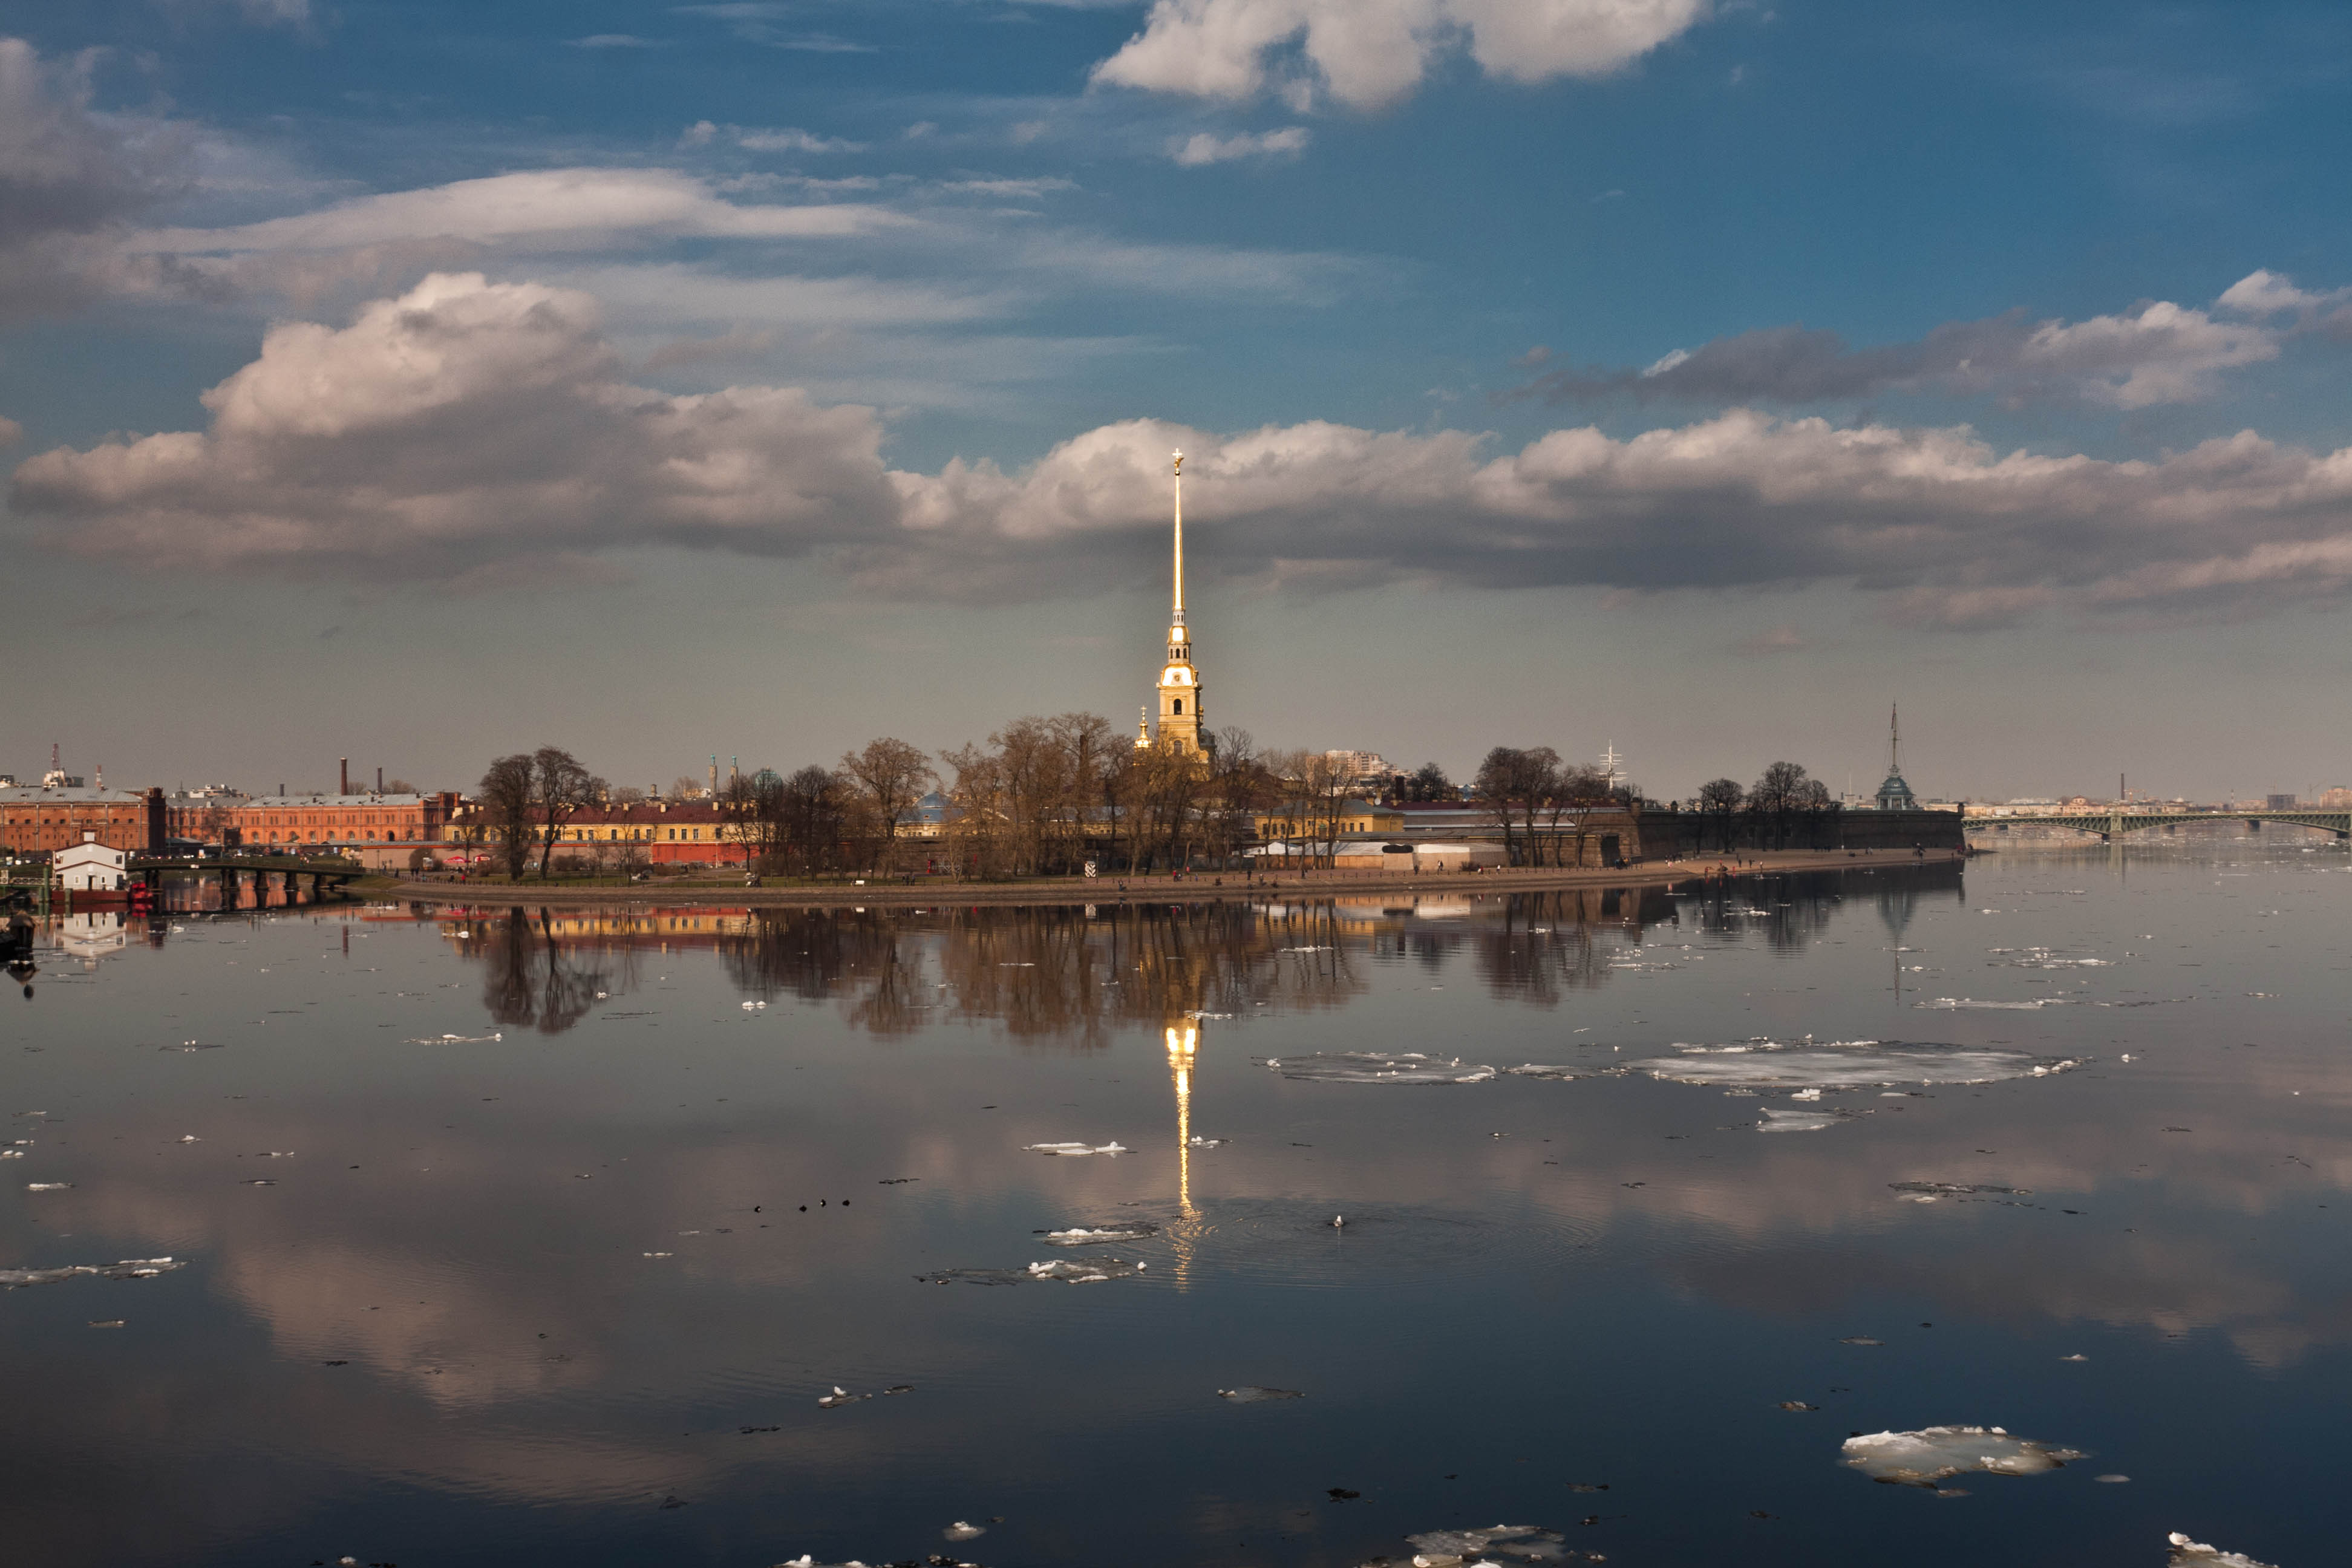
\includegraphics[width=1\textwidth]{boat2.jpg}
          \caption{boat2.jpg}
          \label{fig:boat2}
          \end{figure}
          \begin{figure}[H]
          \centering
          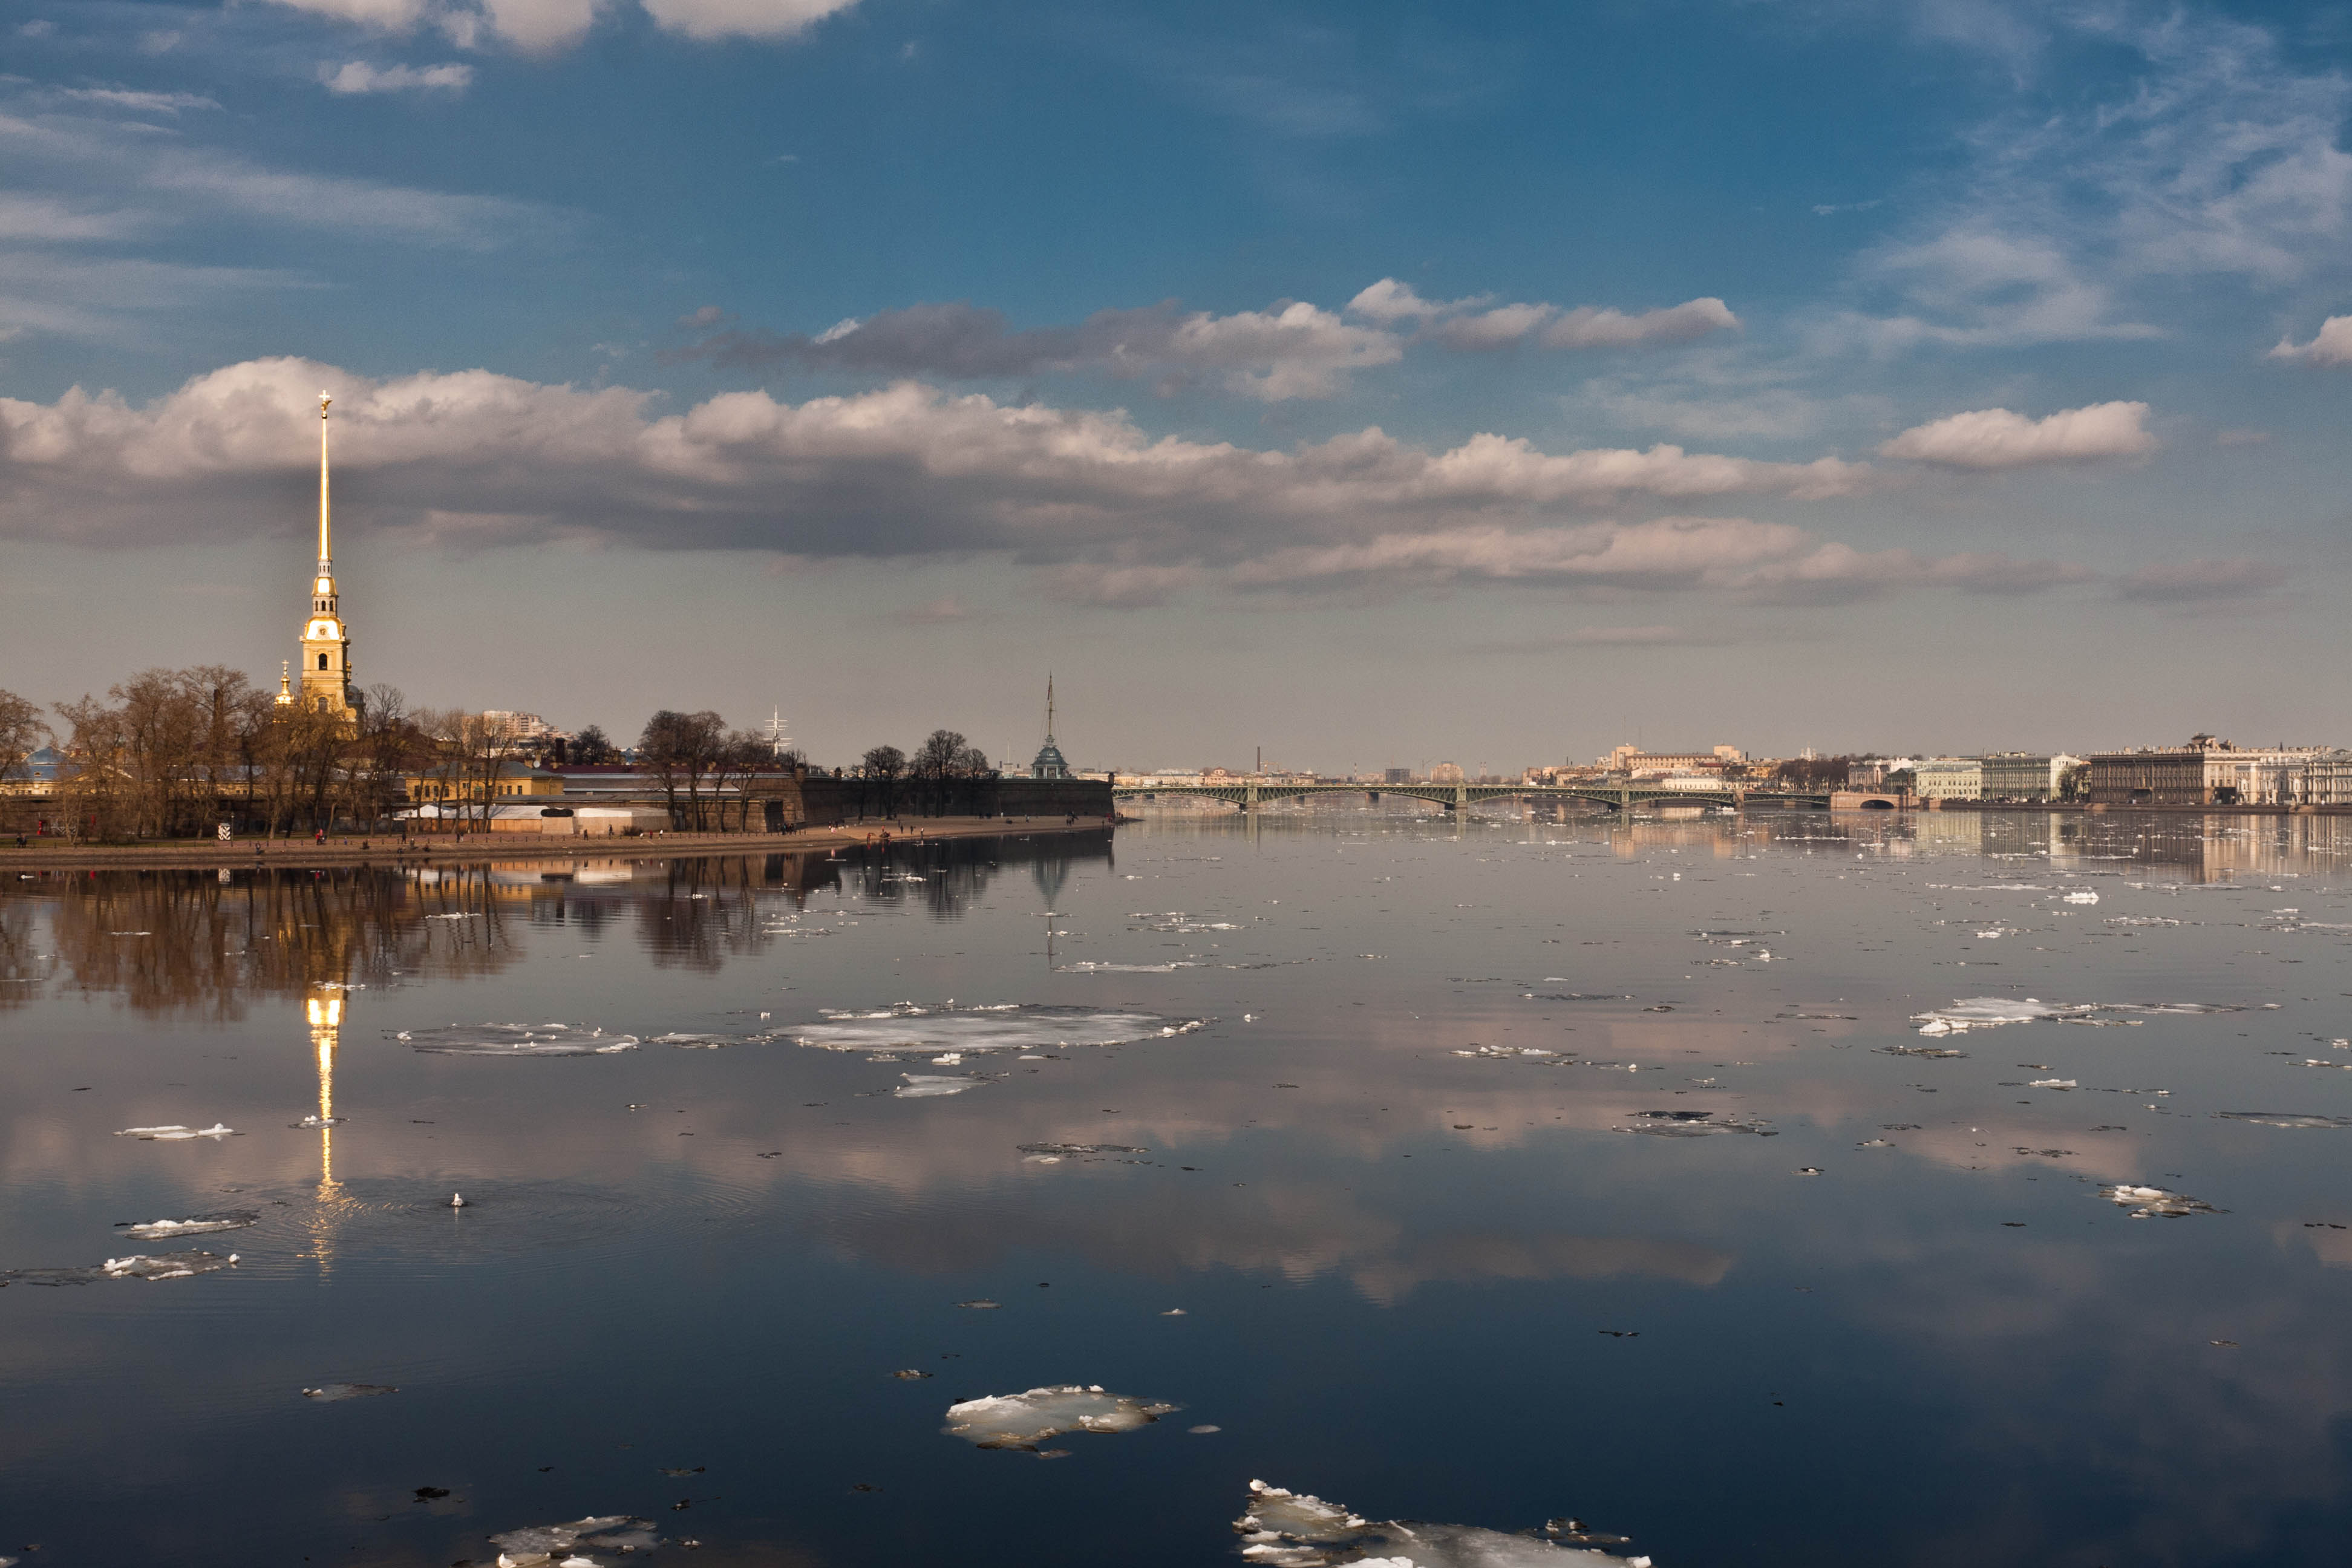
\includegraphics[width=1\textwidth]{boat3.jpg}
          \caption{boat3.jpg}
          \label{fig:boat3}
          \end{figure}
\section{Resulting Image}
The resulting image after image stitching is shown in Figure \ref{fig:resultimg}.
\begin{figure}[H]
          \centering
          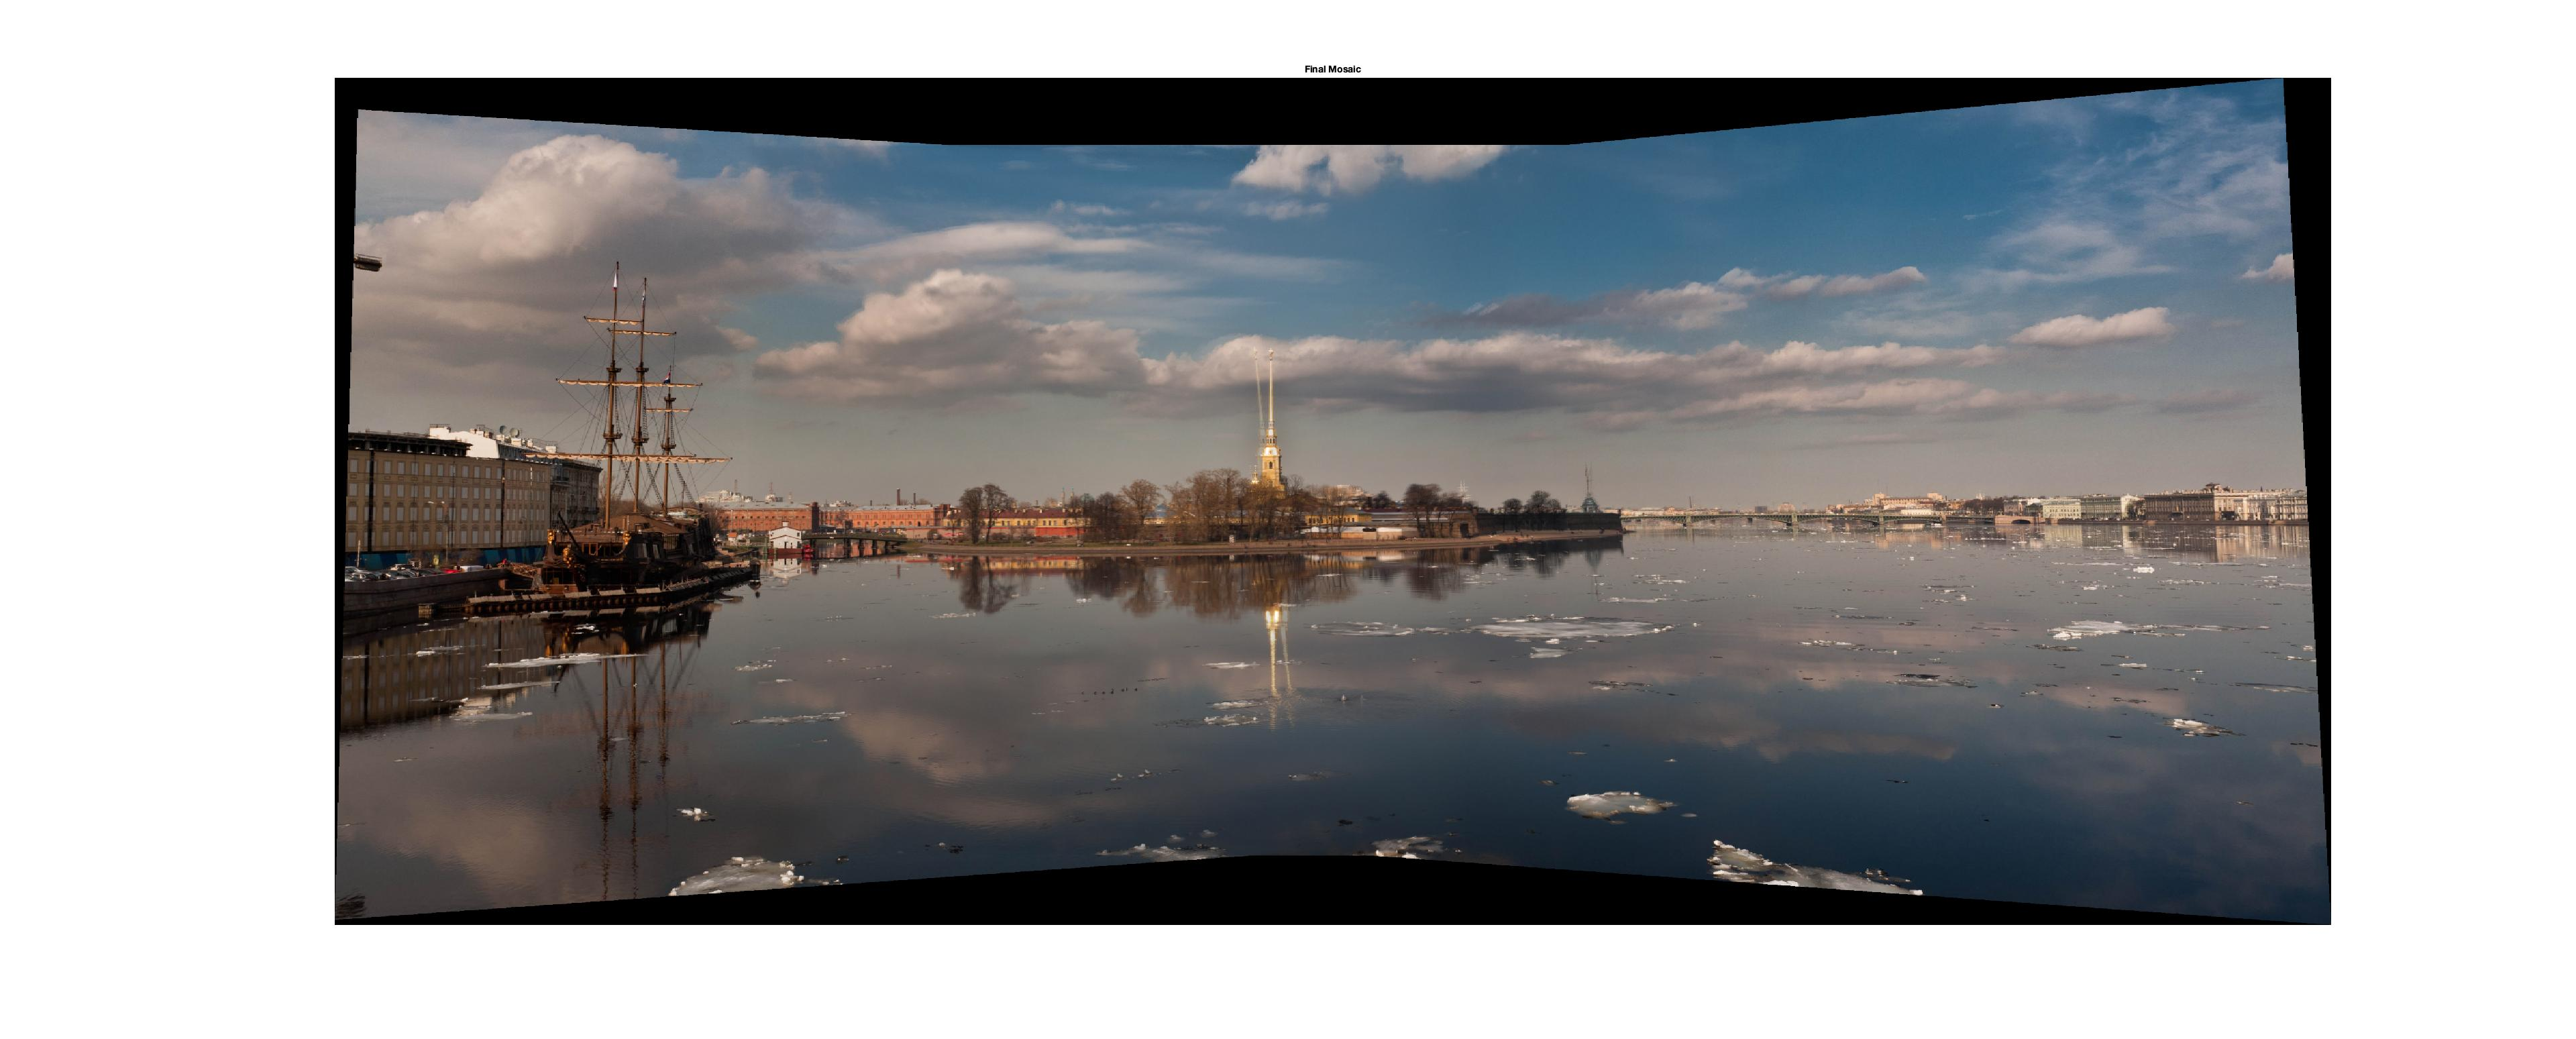
\includegraphics[width=1\textwidth]{resultimg.jpg}
          \caption{Resulting Image}
          \label{fig:resultimg}
          \end{figure}
\section{Results of Corner Detection and Adaptive Non-Maximal Suppression}
\begin{enumerate}
    \item For \texttt{boat1.jpg}, the results are shown in Figure \ref{fig:img1}.\\
        \begin{figure}[H]
          \centering
          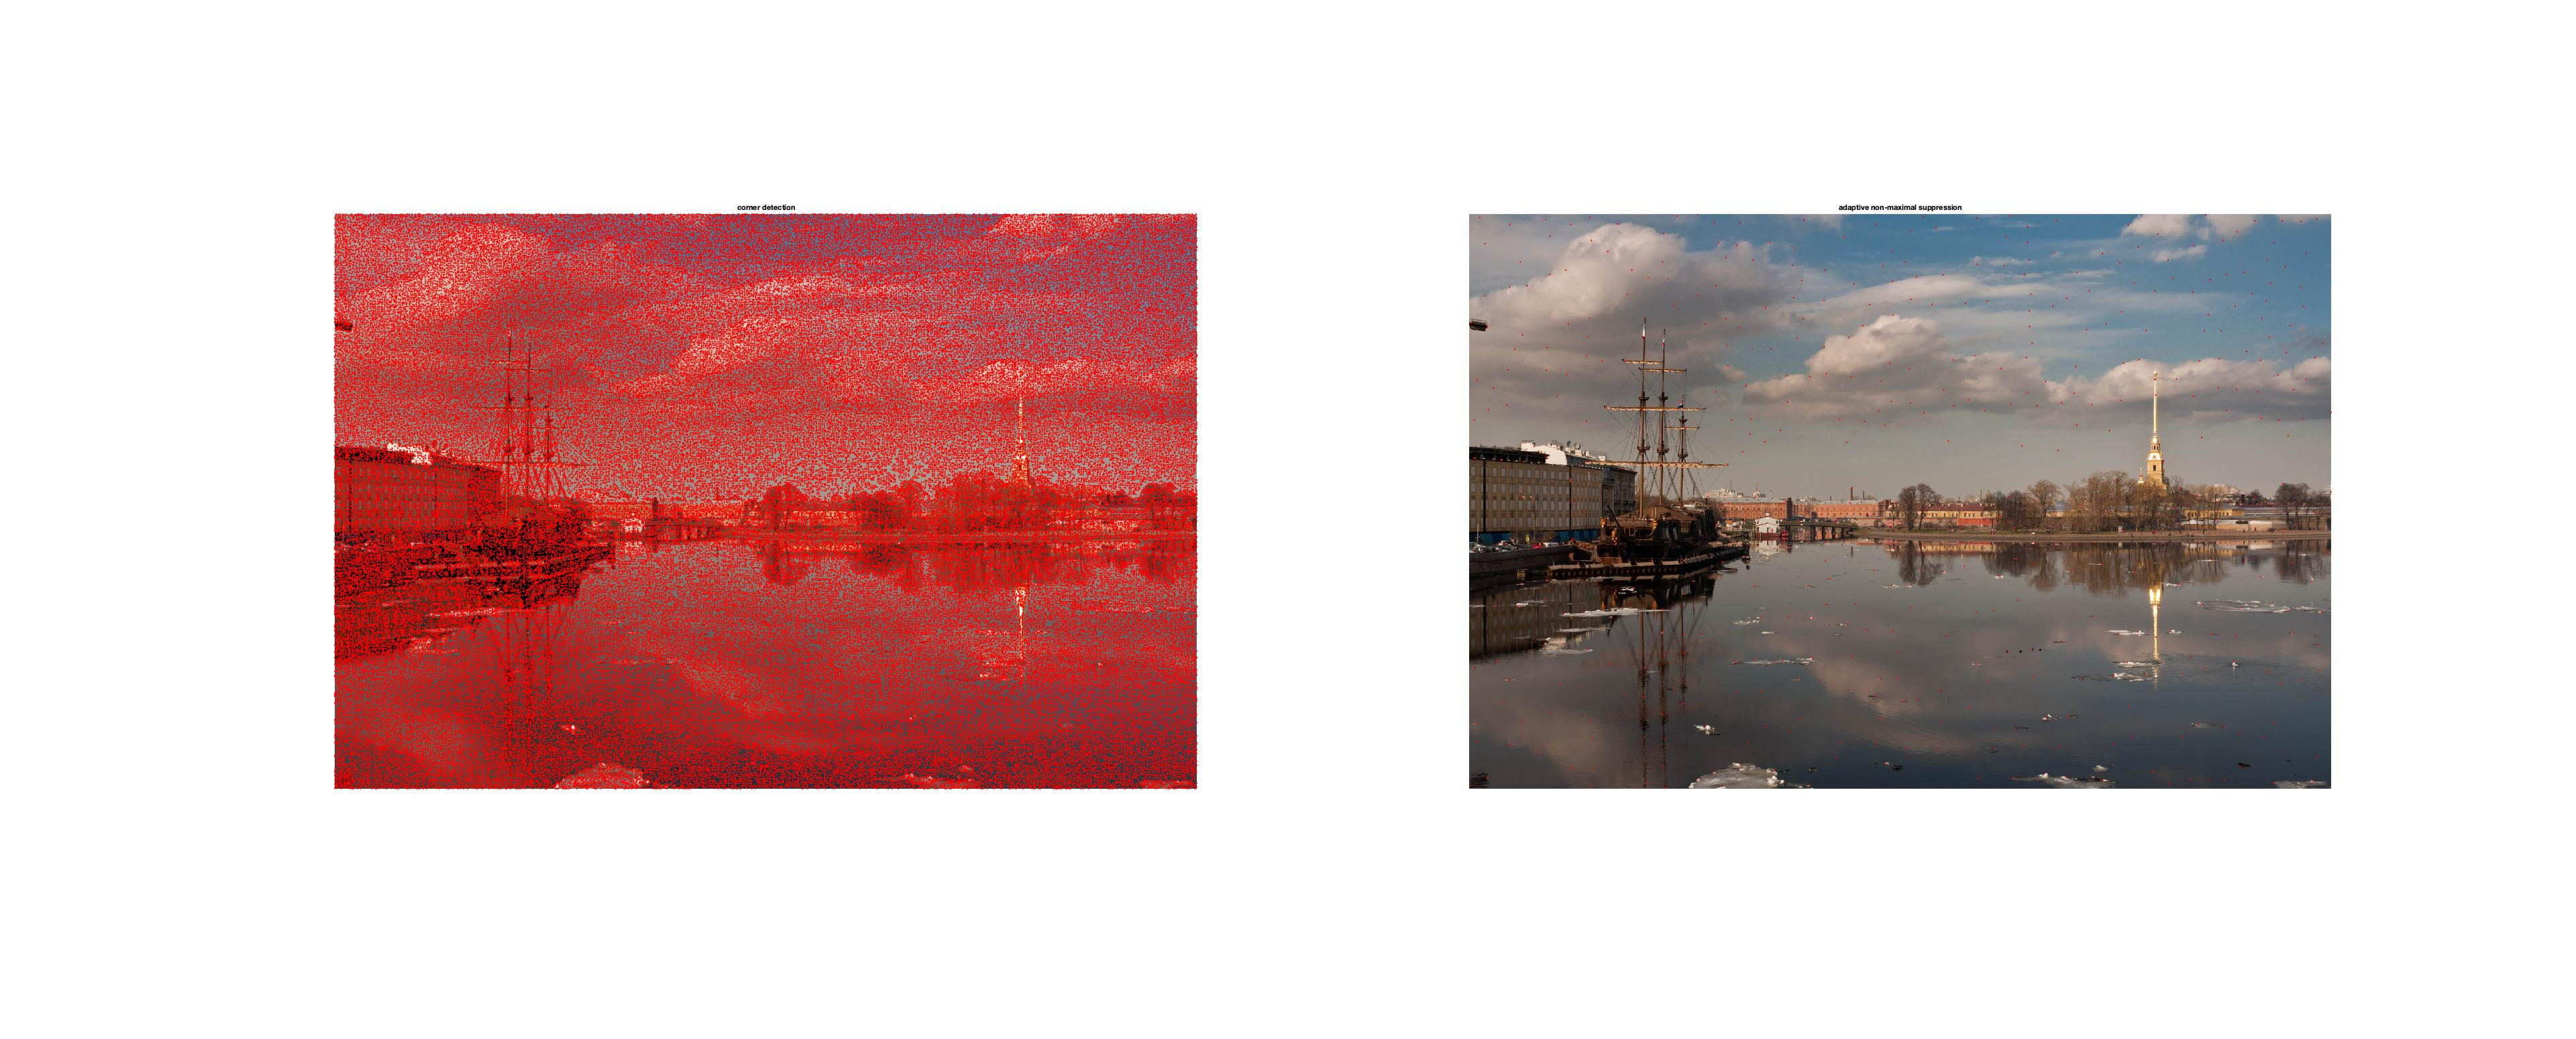
\includegraphics[width=1\textwidth]{img1.jpg}
          \caption{Results of Corner Detection and Adaptive Non-Maximal Suppression of the First Image.}
          \label{fig:img1}
        \end{figure}
        \item For \texttt{boat2.jpg}, the results are shown in Figure \ref{fig:img2}.\\
        \begin{figure}[H]
          \centering
          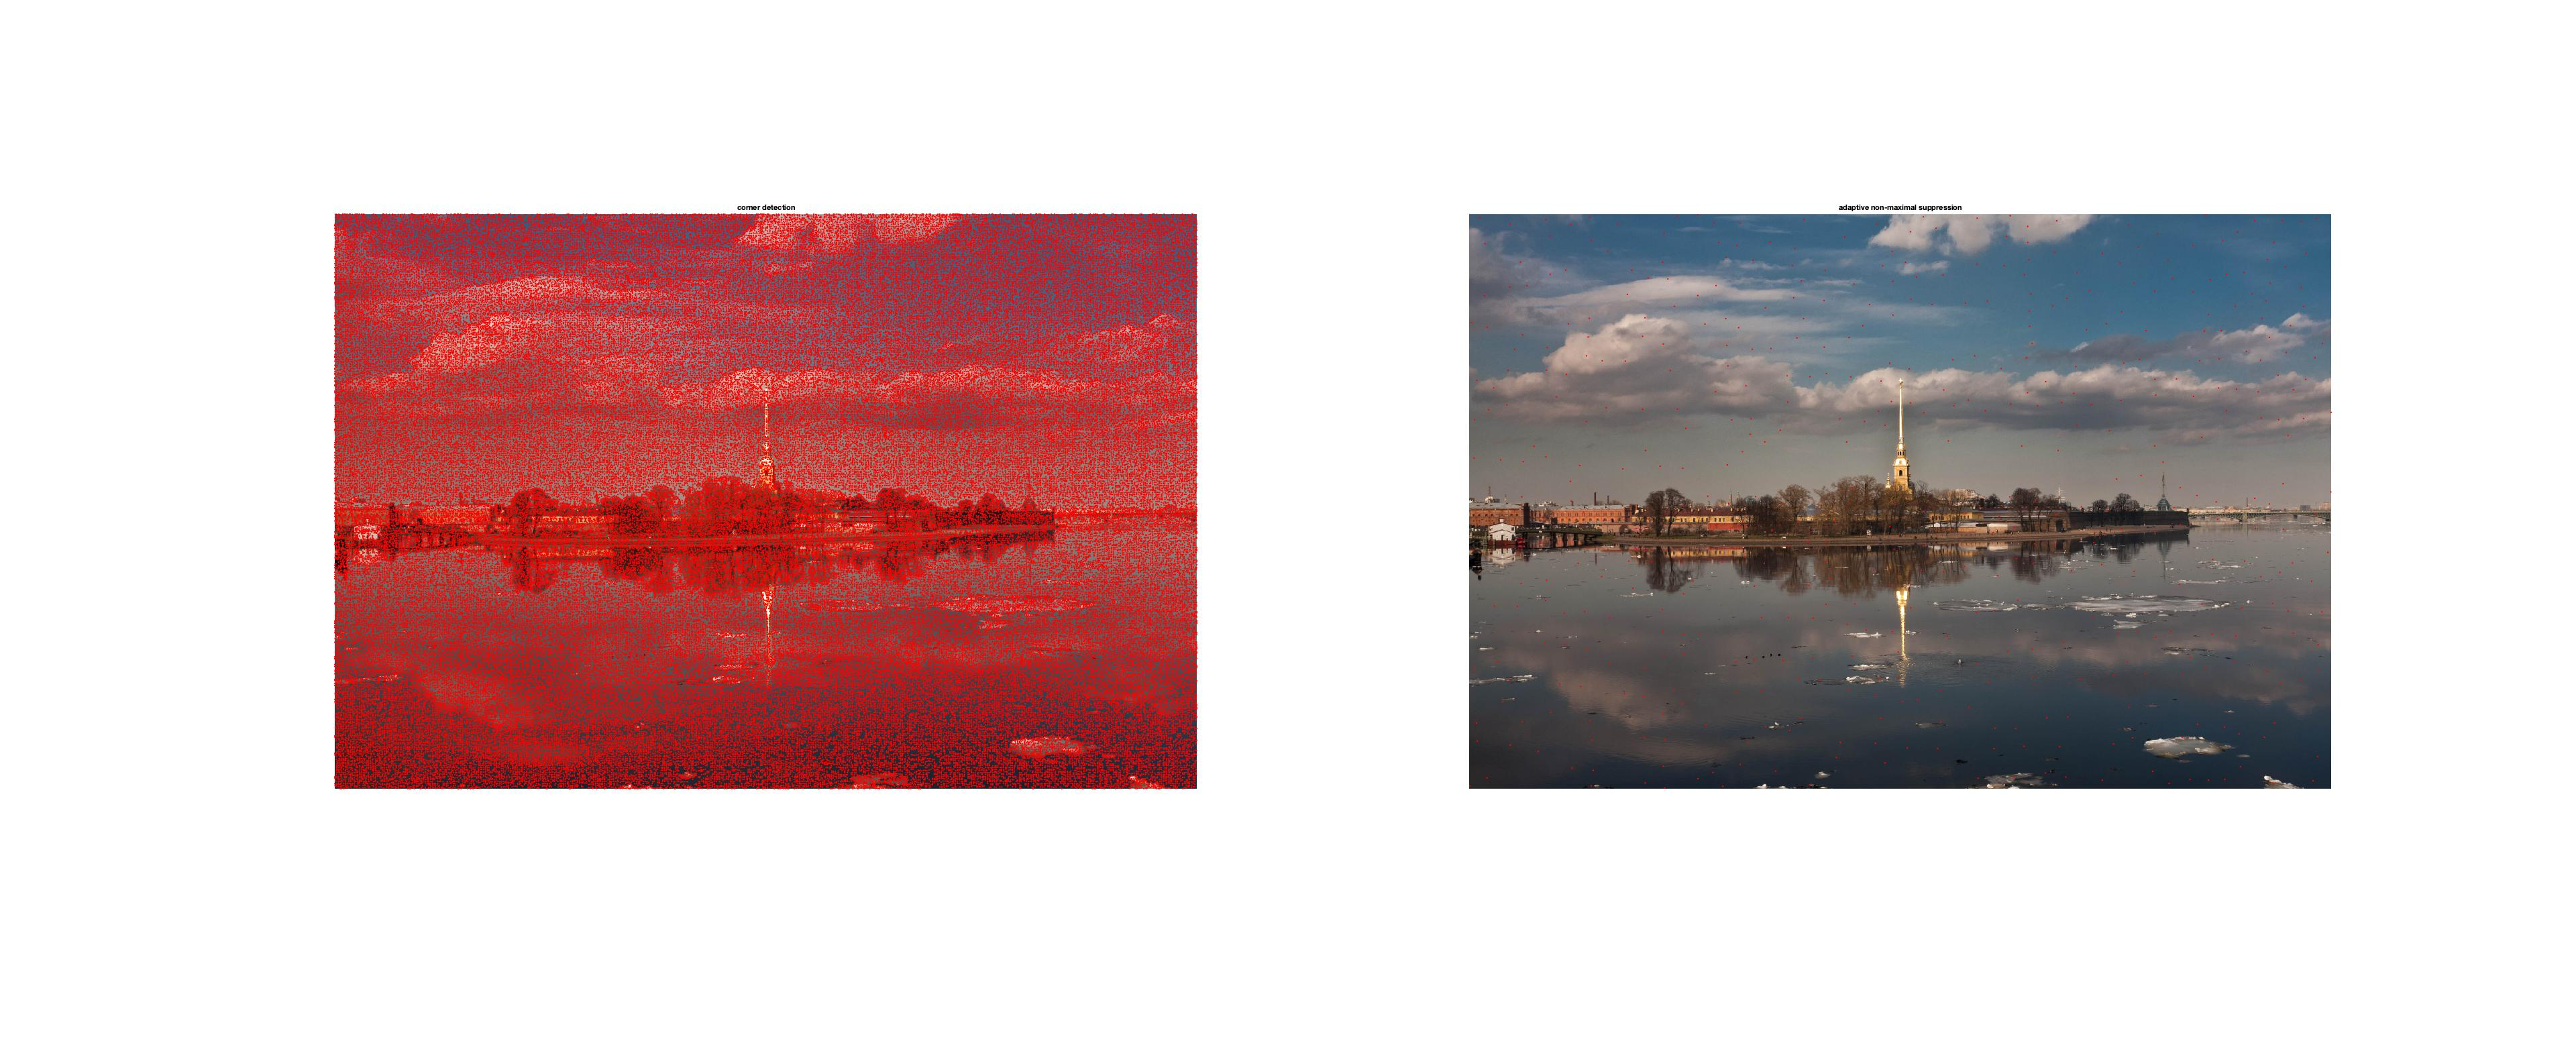
\includegraphics[width=1\textwidth]{img2.jpg}
          \caption{Results of Corner Detection and Adaptive Non-Maximal Suppression of the Second Image.}
          \label{fig:img2}
        \end{figure}
        \item For \texttt{boat3.jpg}, the results are shown in Figure \ref{fig:img3}.\\
        \begin{figure}[H]
          \centering
          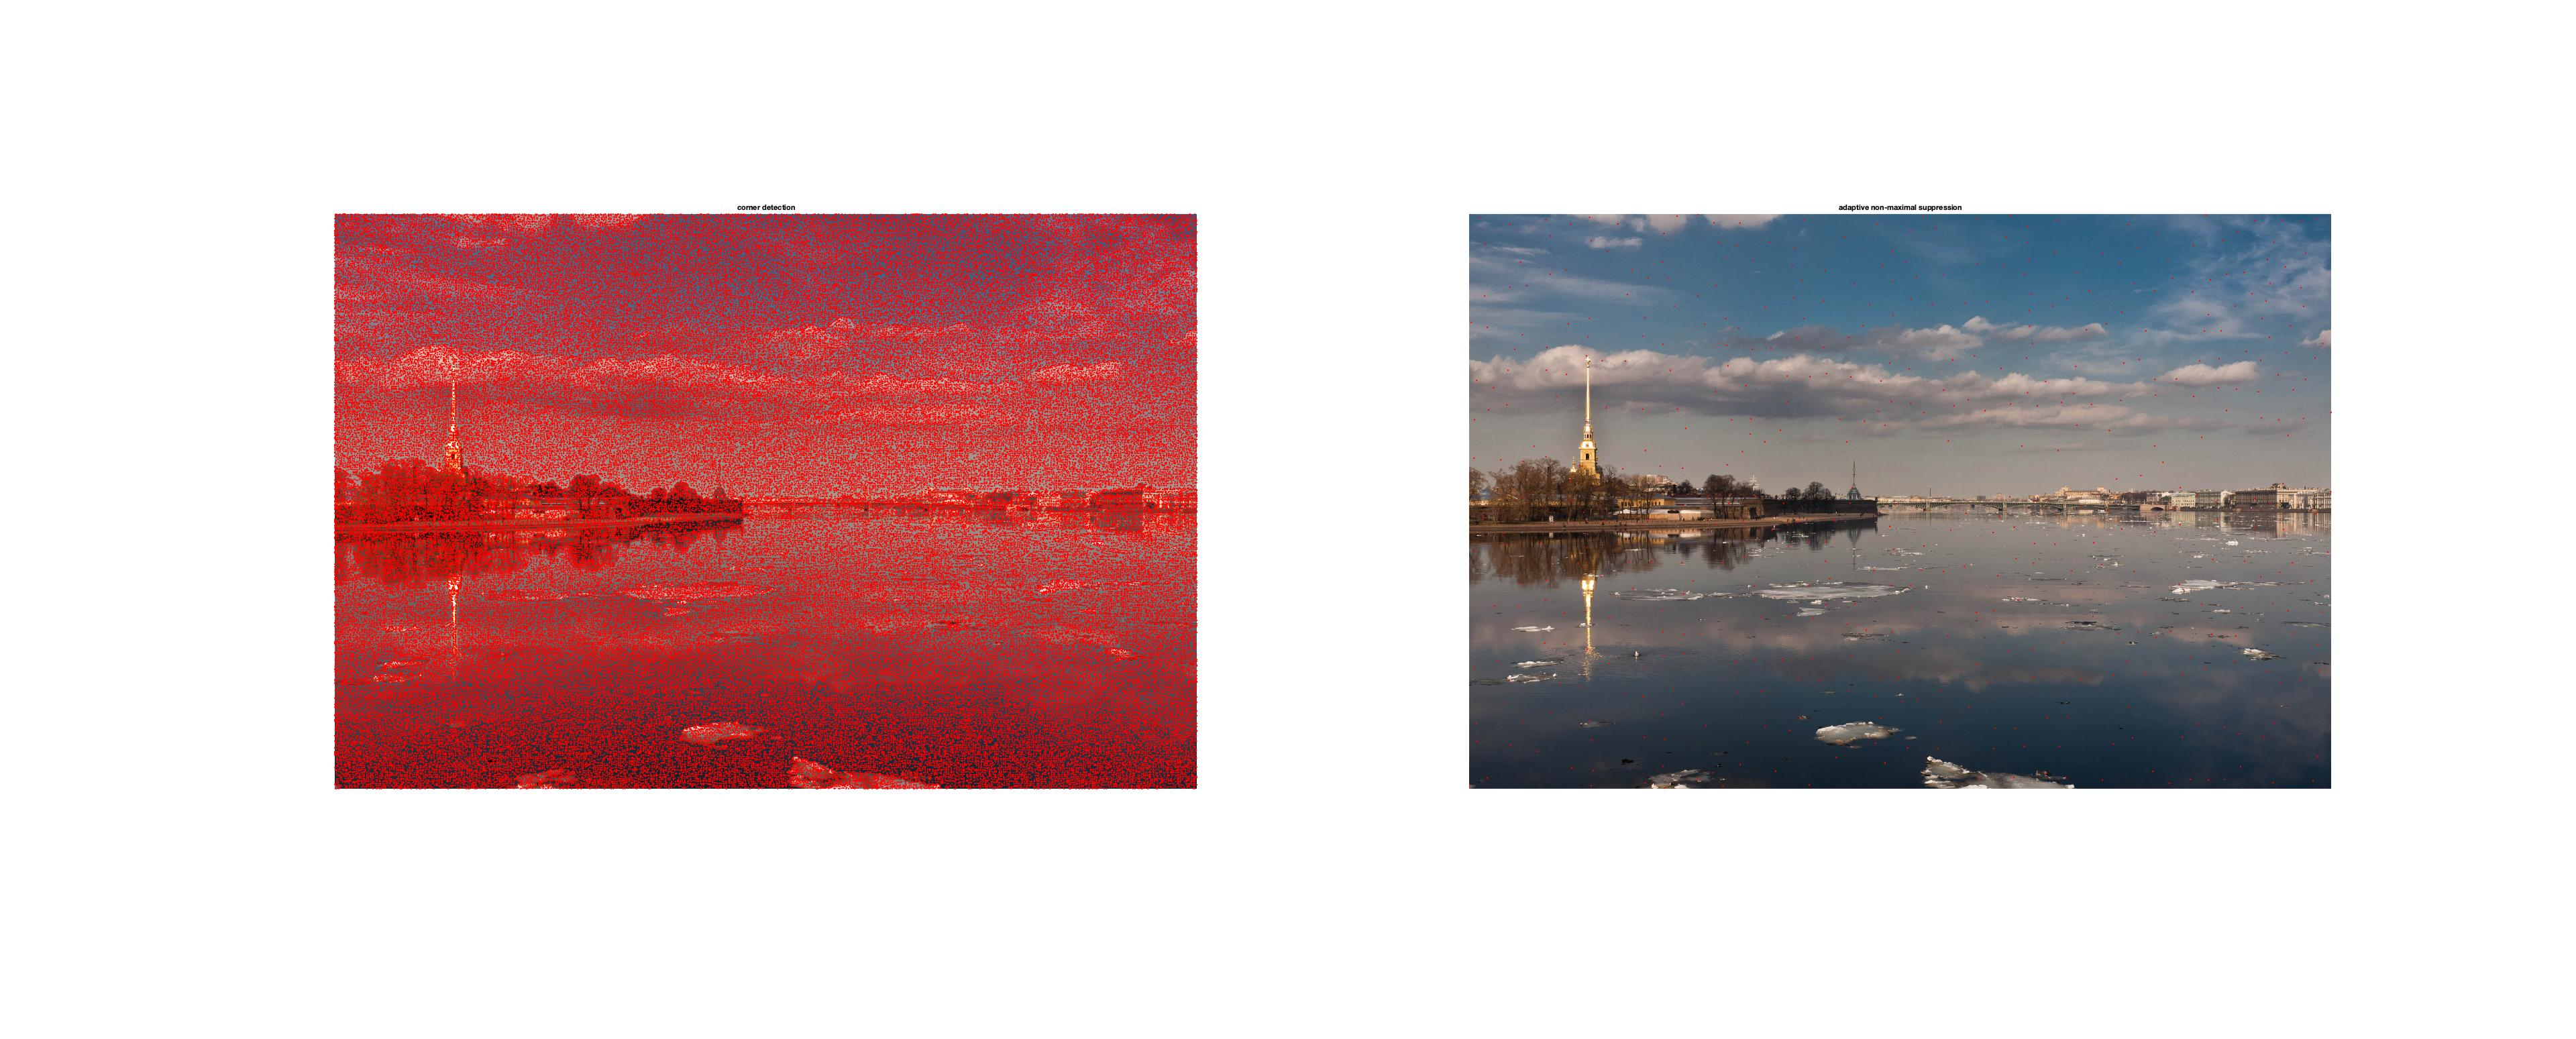
\includegraphics[width=1\textwidth]{img3.jpg}
          \caption{Results of Corner Detection and Adaptive Non-Maximal Suppression of the Third Image.}
          \label{fig:img3}
        \end{figure}
\end{enumerate}
\section{Prior and Post RANSAC Comparison}
\begin{enumerate}
    \item Prior and Post RANSAC of \texttt{boat1.jpg} and \texttt{boat2.jpg}. \\\\The prior-RANSAC is shown in Figure \ref{fig:priorransac1}. The post-RANSAC is shown in Figure \ref{fig:postransac1}.
    \begin{figure}[H]
          \centering
          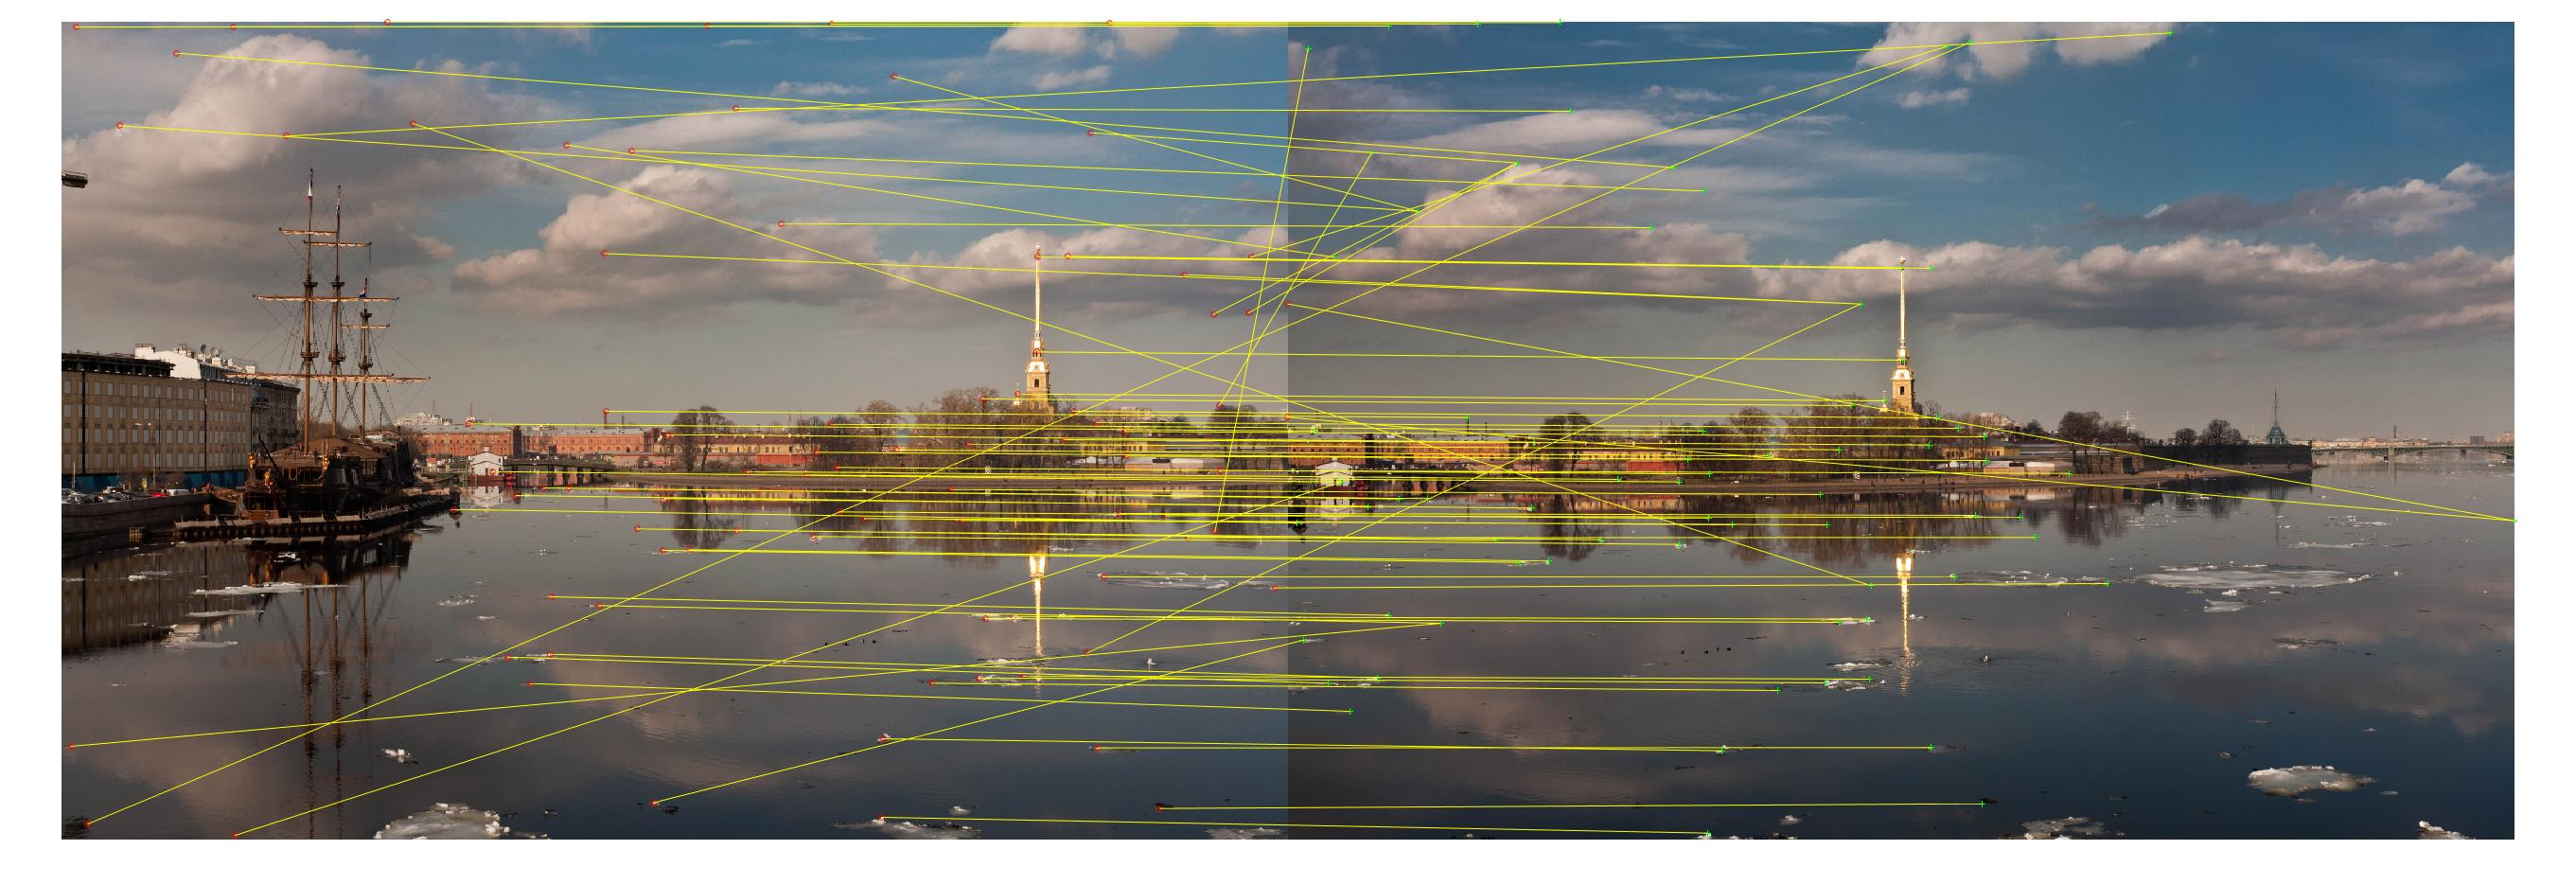
\includegraphics[width=1\textwidth]{priorransac1.jpg}
          \caption{Prior-RANSAC of Image 1 and Image 2.}
          \label{fig:priorransac1}
        \end{figure}
        \begin{figure}[H]
          \centering
          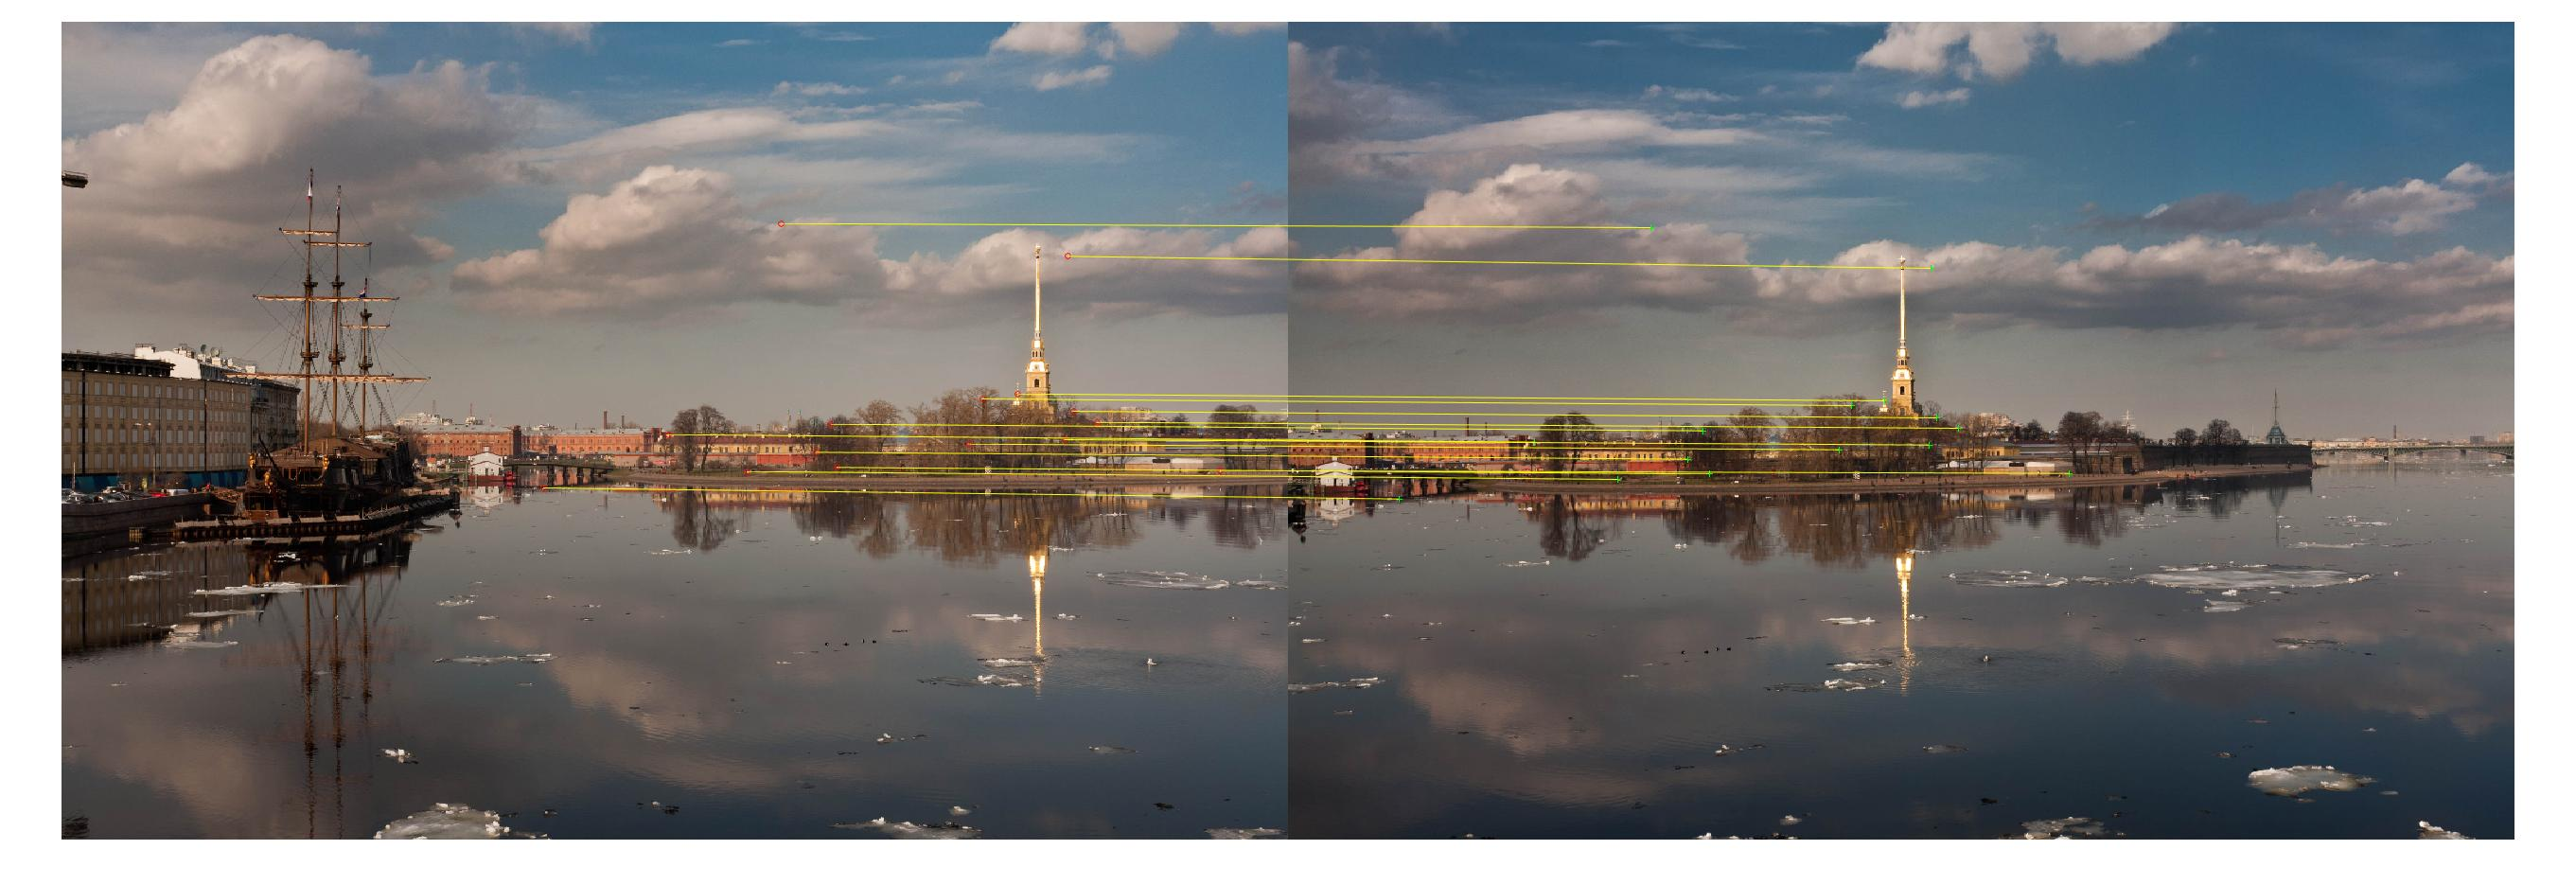
\includegraphics[width=1\textwidth]{postransac1.jpg}
          \caption{Post-RANSAC of Image 1 and Image 2.}
          \label{fig:postransac1}
        \end{figure}
    \item Prior and Post RANSAC of \texttt{boat2.jpg} and \texttt{boat3.jpg}. \\\\The prior-RANSAC is shown in Figure \ref{fig:priorransac2}. The post-RANSAC is shown in Figure \ref{fig:postransac2}.
    \begin{figure}[H]
          \centering
          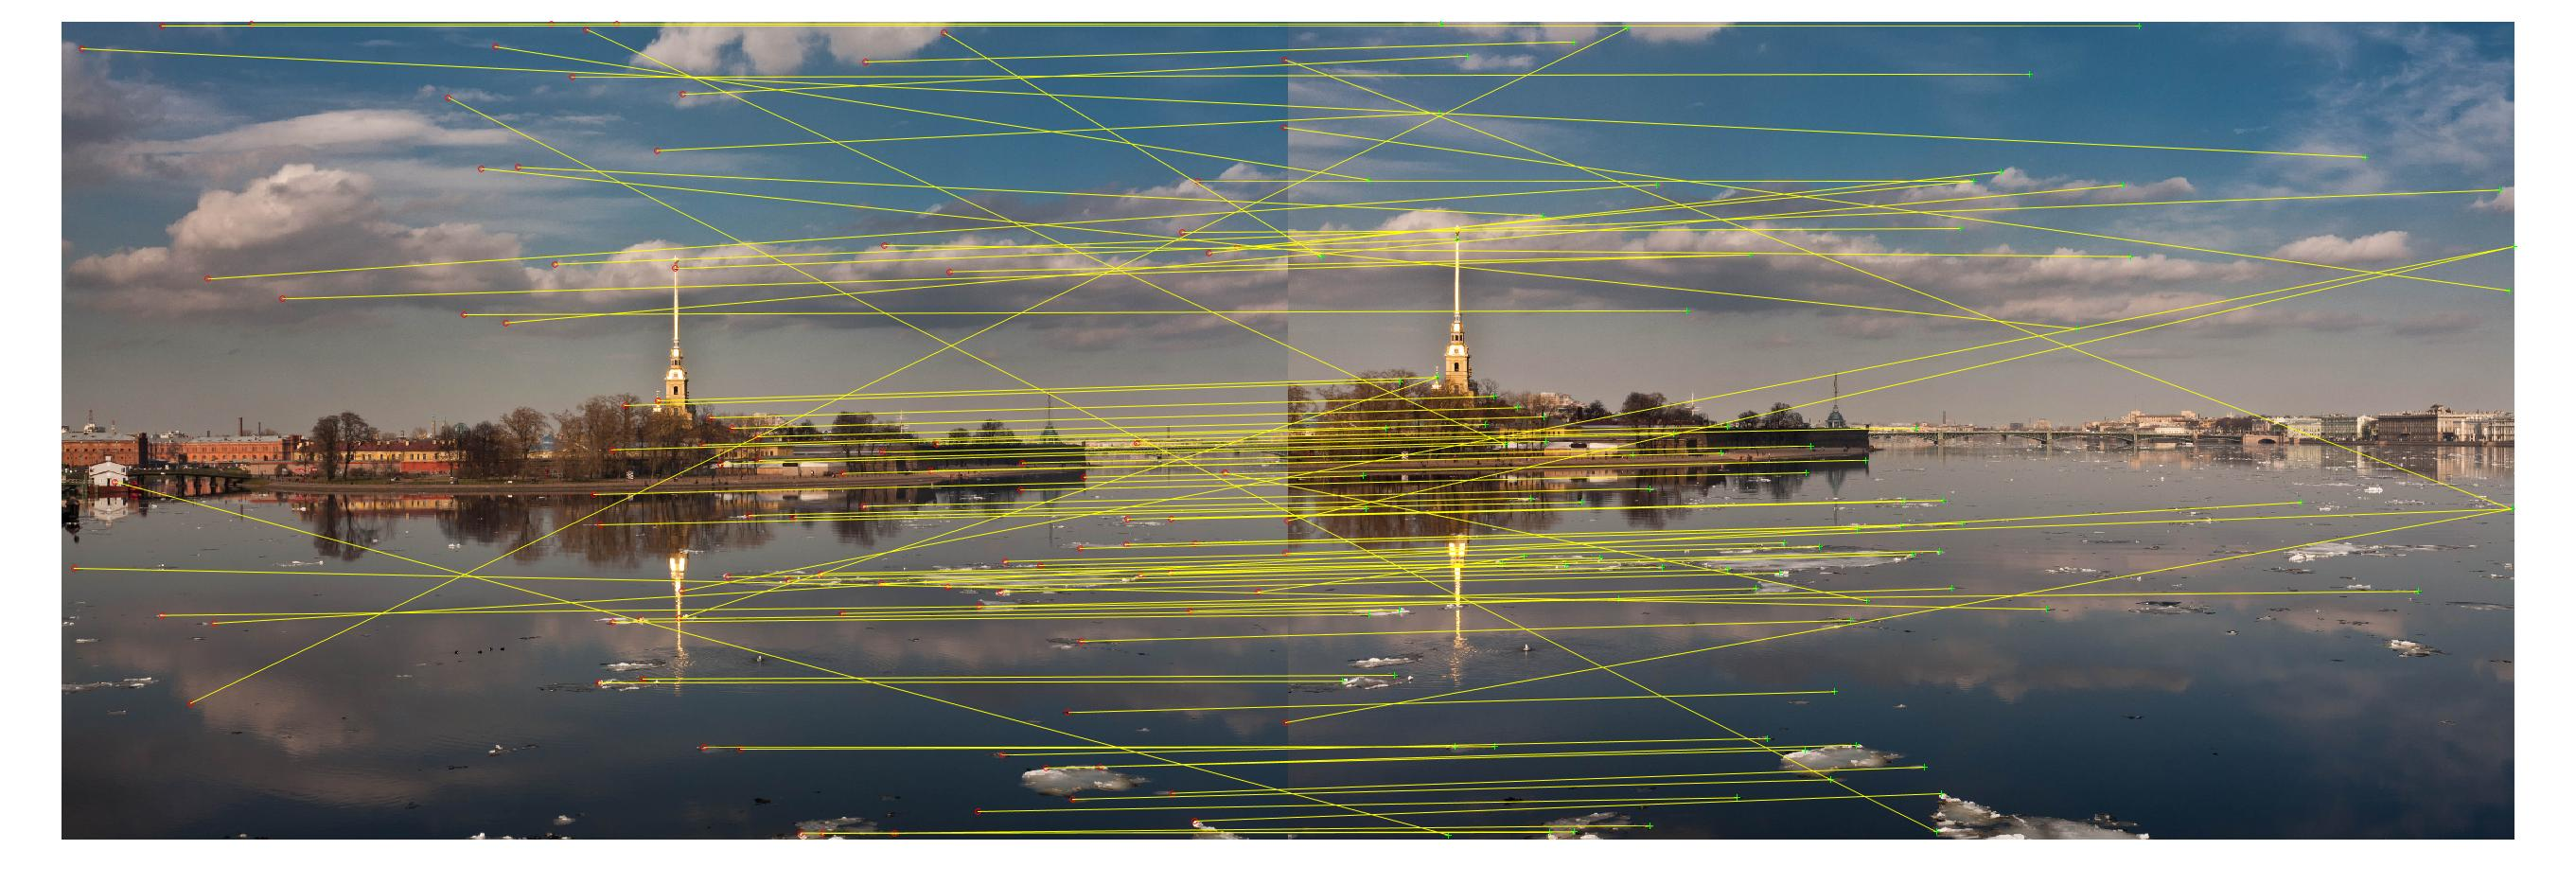
\includegraphics[width=1\textwidth]{priorransac2.jpg}
          \caption{Prior-RANSAC of Image 2 and Image 3.}
          \label{fig:priorransac2}
        \end{figure}
        \begin{figure}[H]
          \centering
          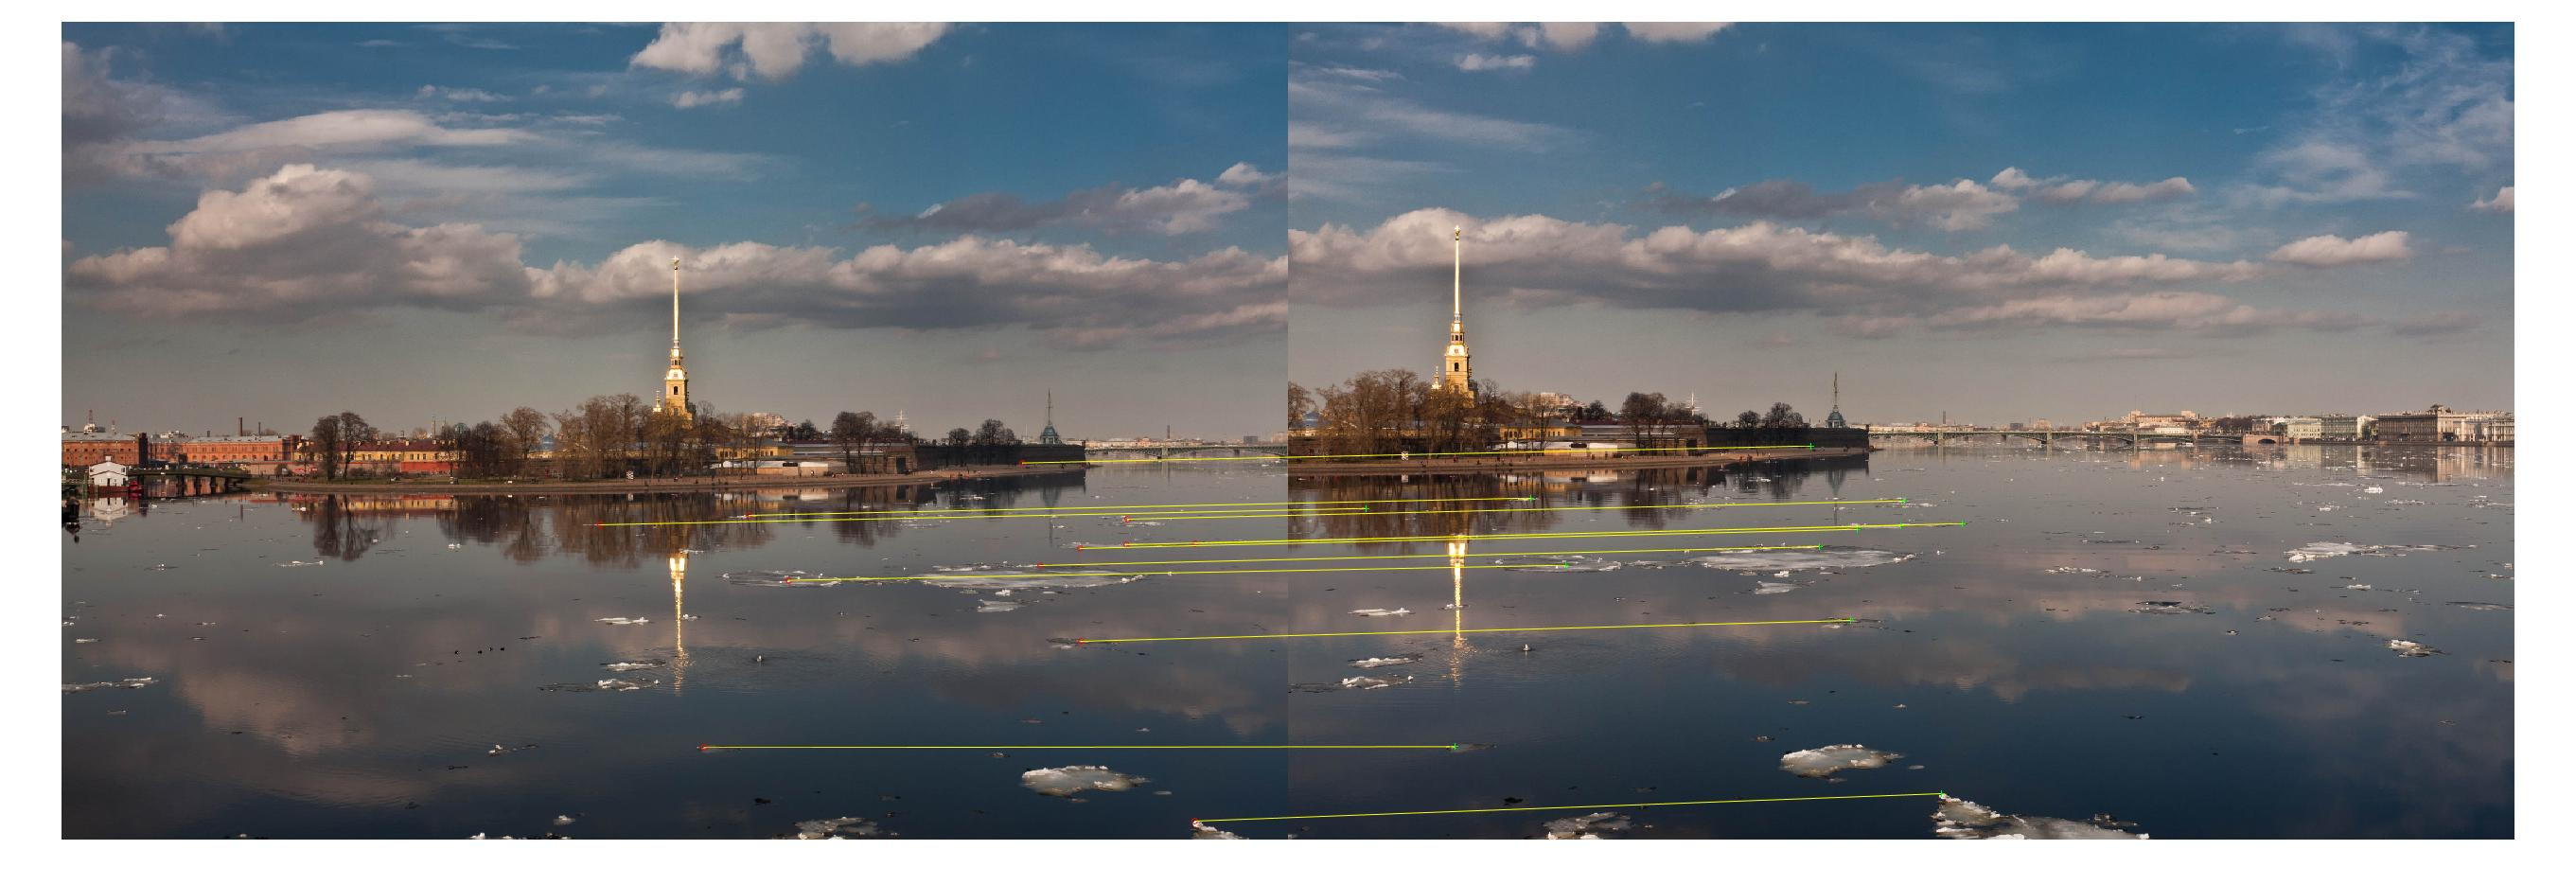
\includegraphics[width=1\textwidth]{postransac2.jpg}
          \caption{Post-RANSAC of Image 2 and Image 3.}
          \label{fig:postransac2}
        \end{figure}
\end{enumerate}
\section{References}
\begin{enumerate}
  \item \url{https://www.mathworks.com/help/vision/examples/feature-based-panoramic-image-stitching.html}
\end{enumerate}
\end{document}
